\documentclass{beamer}

\usefonttheme{professionalfonts} % using non standard fonts for beamer
\usefonttheme{serif} % default family is serif

\usepackage{hyperref}
%\usepackage{minted}
\usepackage{animate}
\usepackage{graphicx}
\def\Put(#1,#2)#3{\leavevmode\makebox(0,0){\put(#1,#2){#3}}}
\usepackage{color}
\usepackage{tikz}
\usepackage{amssymb}
\usepackage{enumerate}


\newcommand\blfootnote[1]{%

  \begingroup

  \renewcommand\thefootnote{}\footnote{#1}%

  \addtocounter{footnote}{-1}%

  \endgroup

}

\makeatletter

%%%%%%%%%%%%%%%%%%%%%%%%%%%%%% Textclass specific LaTeX commands.

 % this default might be overridden by plain title style

 \newcommand\makebeamertitle{\frame{\maketitle}}%

 % (ERT) argument for the TOC

 \AtBeginDocument{%

   \let\origtableofcontents=\tableofcontents

   \def\tableofcontents{\@ifnextchar[{\origtableofcontents}{\gobbletableofcontents}}

   \def\gobbletableofcontents#1{\origtableofcontents}

 }

%%%%%%%%%%%%%%%%%%%%%%%%%%%%%% User specified LaTeX commands.

\usetheme{Malmoe}

% or ...

\useoutertheme{infolines}

\addtobeamertemplate{headline}{}{\vskip2pt}

\setbeamercovered{transparent}

% or whatever (possibly just delete it)

\makeatother

\begin{document}
\title[PFLOCK report]{PFLOCK Report}
\author[AC]{Andres Calderon}
\institute[Fall'19]{University of California, Riverside}
\makebeamertitle
\newif\iflattersubsect

\AtBeginSection[] {
    \begin{frame}<beamer>
    \frametitle{Outline} 
    \tableofcontents[currentsection]  
    \end{frame}
    \lattersubsectfalse
}

\AtBeginSubsection[] {
    \begin{frame}<beamer>
    \frametitle{Outline} 
    \tableofcontents[currentsubsection]  
    \end{frame}
}

\begin{frame}{Pattern enumerator}
    {\small Example 1 ($\delta=3, \mu=2$)}
    \centering
    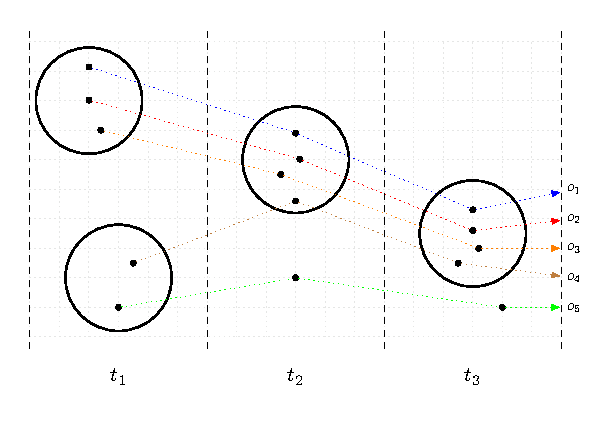
\includegraphics[width=0.9\textwidth]{Figures/Trajs01}
\end{frame}
\begin{frame}{Pattern enumerator}
    {\small Example 1 ($\delta=3, \mu=2$)}
    \centering
    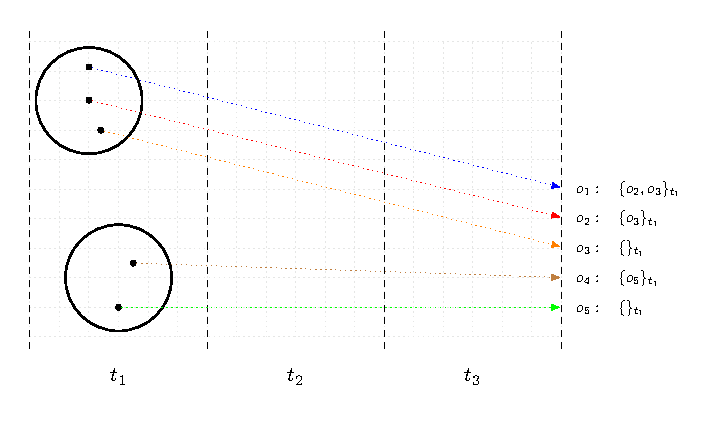
\includegraphics[width=\textwidth]{Figures/Trajs01t1}
\end{frame}
\begin{frame}{Pattern enumerator}
    {\small Example 1 ($\delta=3, \mu=2$)}
    \centering
    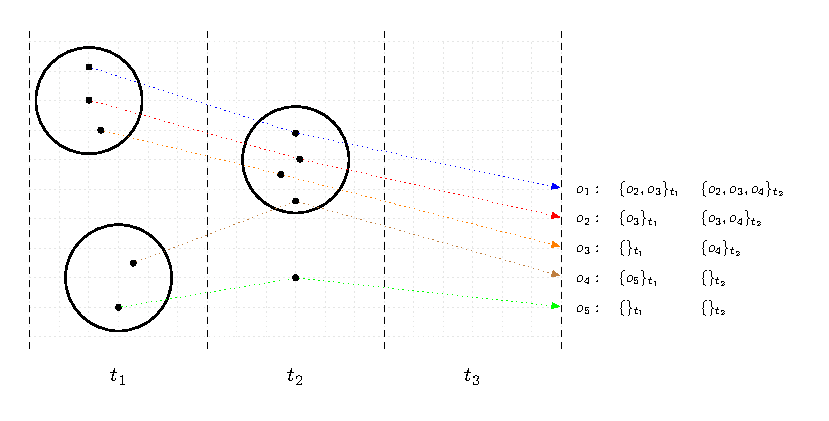
\includegraphics[width=\textwidth]{Figures/Trajs01t2}
\end{frame}
\begin{frame}{Pattern enumerator}
    {\small Example 1 ($\delta=3, \mu=2$)}
    \centering
    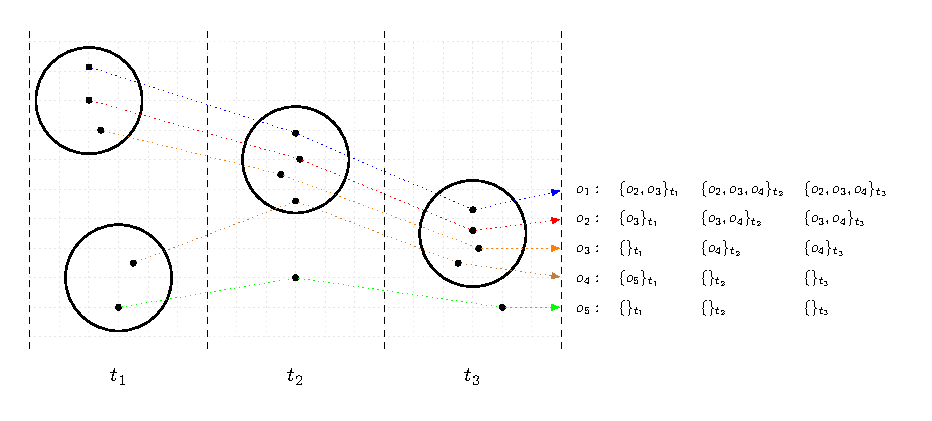
\includegraphics[width=\textwidth]{Figures/Trajs01t3}
\end{frame}
\begin{frame}{Pattern enumerator}
    {\small Example 1 ($\delta=3, \mu=2$): Redundant flocks}
    \centering
    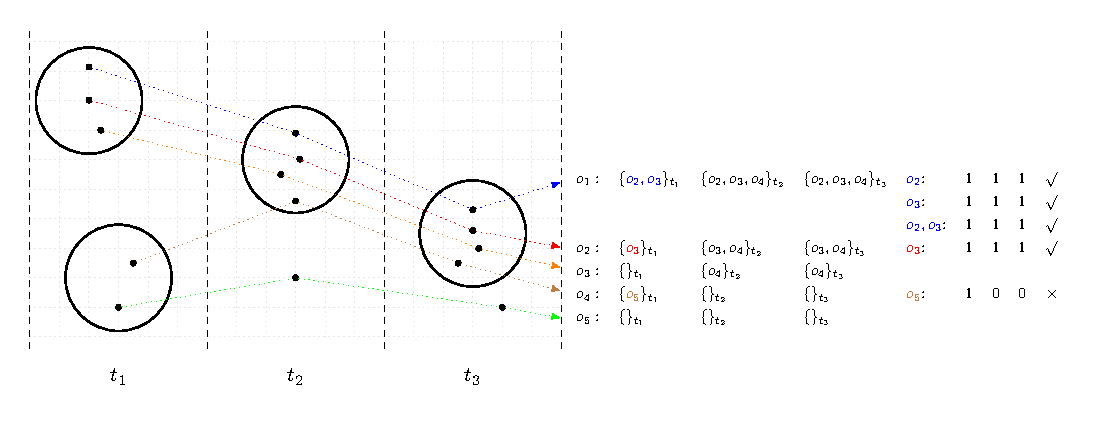
\includegraphics[width=\textwidth]{Figures/Trajs01t3Bits}
\end{frame}

\begin{frame}{Pattern enumerator}
    {\small Example 2 ($\delta=3, \mu=3$)}
    \centering
    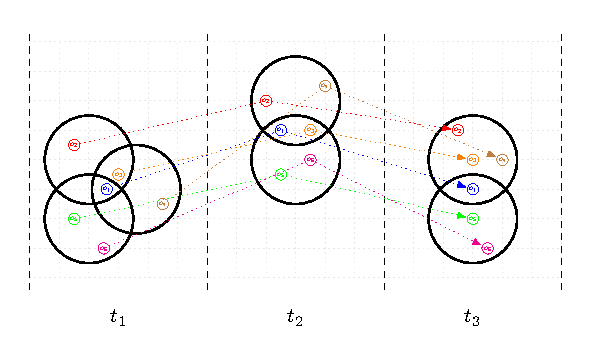
\includegraphics[width=\textwidth]{Figures/Trajs02}
\end{frame}
\begin{frame}{Pattern enumerator}
    {\small Example 2 ($\delta=3, \mu=3$): Overlapping}
    \centering
    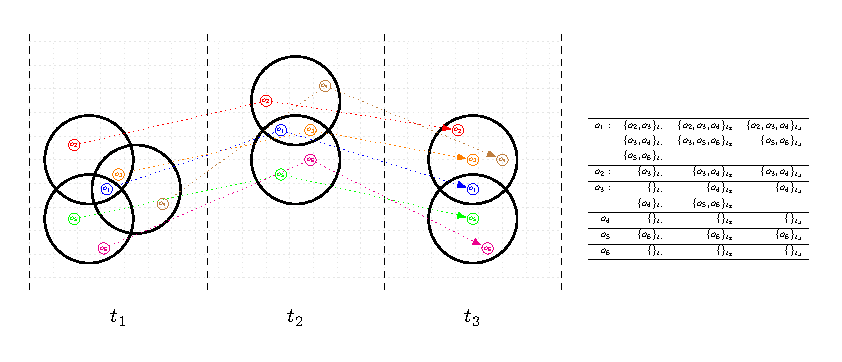
\includegraphics[width=\textwidth]{Figures/Trajs02Partitions}
\end{frame}
\begin{frame}{Pattern enumerator}
    {\small Combinations}
    \centering
    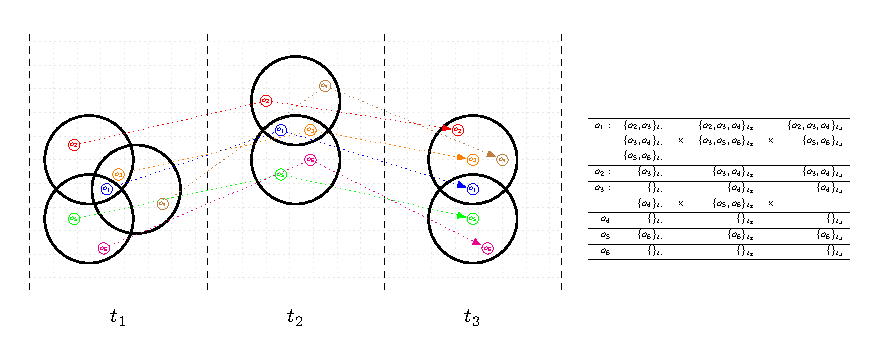
\includegraphics[width=\textwidth]{Figures/Trajs02Combinations}
\end{frame}
\begin{frame}{Pattern enumerator}
    {\small Maximal patterns}
    \centering
    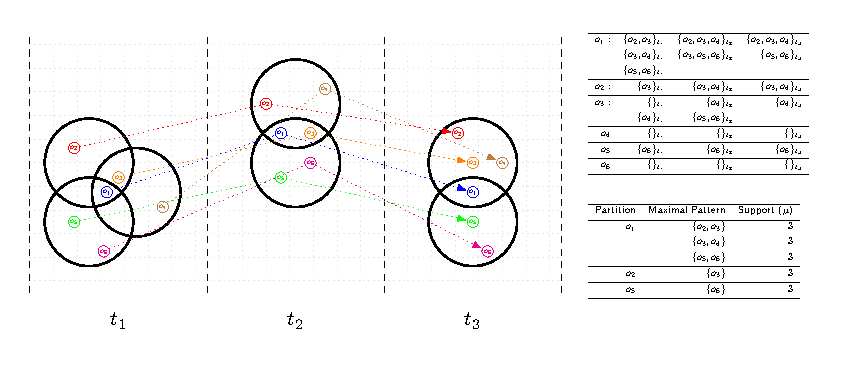
\includegraphics[width=\textwidth]{Figures/Trajs02MaxPatterns}
\end{frame}

\begin{frame}{What is next?}
    \begin{itemize}
        \item Explore volumes.
        \item Extent pattern enumeration with one of the alternatives.
        \item Perform tests.
    \end{itemize}
\end{frame}

\end{document}
